% Created 2019-03-25 Mon 13:22
% Intended LaTeX compiler: pdflatex
\documentclass[11pt]{article}
\usepackage[utf8]{inputenc}
\usepackage[T1]{fontenc}
\usepackage{graphicx}
\usepackage{grffile}
\usepackage{longtable}
\usepackage{wrapfig}
\usepackage{rotating}
\usepackage[normalem]{ulem}
\usepackage{amsmath}
\usepackage{textcomp}
\usepackage{amssymb}
\usepackage{capt-of}
\usepackage{hyperref}
\usepackage{amsmath}
\usepackage{xcolor}
\PassOptionsToPackage{hyperref,x11names}{xcolor}
\definecolor{electricblue}{HTML}{05ADF3}
\usepackage{tocloft}
\sloppy
\renewcommand{\cftsecleader}{\cftdotfill{\cftdotsep}}
\pagenumbering{gobble}
\setlength\parindent{0pt}
\setlength\parskip{12pt}
\usepackage[breaklinks=true,linktocpage,xetex]{hyperref}
\hypersetup{colorlinks, citecolor=blue,filecolor=blue,linkcolor=blue,urlcolor=blue}
\date{}
\title{Using Cognitive Communications to Increase the Operational Value of Collaborative Networks of Satellites}
\hypersetup{
 pdfauthor={Ryan},
 pdftitle={Using Cognitive Communications to Increase the Operational Value of Collaborative Networks of Satellites},
 pdfkeywords={},
 pdfsubject={},
 pdfcreator={Emacs 26.1 (Org mode 9.1.9)},
 pdflang={English}}
\begin{document}

\maketitle
\section*{Abstract}
\label{sec:org7ab0300}

Future Earth-observing systems will involve distributed missions of autonomous
and heterogeneous spaceborne sensor networks.  Future sensor webs will occupy a
more complex decision space and will be capable of adaptive decisions and
collaborative networking.  These capabilities must be utilized to increase a
network's operational value and to reduce human involvement in high-level
communications decisions.  Developing this technology may be greatly accelerated
by machine learning techniques and cognitive communications algorithms.  The
following research describes the development and analysis of simulated
observing-systems which employ a cognitive communications model.  Results from
these simulations provide training data for machine learning models to explore
the new decision space.

\section*{I. INTRODUCTION}
\label{sec:orgdd8b396}

It is envisioned that NASA's future space systems will be composed of large,
inhomogeneous networks of small satellites and autonomous platforms.  These
resource constrained systems, carrying an array of different instruments, will
be expected to operate autonomously and collaboratively to achieve mission and
science goals.  Unfortunately, current and near-future inter-satellite
communications are highly constrained in terms of link availability,
reliability, power and bandwidth.  Although future technologies (such as free
space optical links) may alleviate some constraints, it is expected that future
instruments will rapidly expand in both data volume and sensor
reconfigurability.  In this way, it is not sufficient to simply increase the
capabilities of the communication links.  Rather, it is also necessary to
improve the complex decision making that communication systems perform, such as
deciding when to transmit, what information is valuable to nodes of the network,
and how to adapt local operations following the reception of new information.

Recently, cognitive space communication algorithms have been proposed as a
solution to address the complexity of future inter-satellite communication
systems.  Typically, these cognitive algorithms have tried to address
communications at a low level and include decision making regarding modulation,
power and bandwidth, and error rate.  However, it is reasonable to expect that
cognition may also offer an improvement in the complex, higher level decisions
of communication in the context of mission and science objectives.  At this
level, cognition is applied to the operation of the network with the decision
making primarily influenced by the constraints of the space communication
network links.

In this work, we show results of simulation studies to explore the advantages
that cognition could offer for collaborative small-satellite networks.  Under a
NASA Advanced Information System Technology program, we are currently developing
an open-source C++ library for the simulation of autonomous and collaborative
networks of adaptive sensors.  This library and accompanying utilities allow for
the efficient simulation of networks of satellites with realistic constraints in
communication, power, and measurements.  A key focus of this software is the
simulation of sensors that operate adaptively.  Adaptive sensors must make
intelligent decisions regarding their configuration based on their own
measurements as well as the measurements provided by other sensors in a network.
However, the extreme complexity of the decision space makes the development of
optimal decision-making systems very difficult.  Thus, an approach based on
cognition could offer an appealing solution.  We investigate how our simulation
tools could be useful for production of large training datasets that capture the
operation of collaborative, adaptive networks of small satellites.  We then
investigate how such a dataset could be combined with machine learning
techniques to train neural networks that could make intelligent decisions about
when and what to communicate.  Results from our investigation will be presented,
and the applicability of these methods to future cognitive space communication
will be discussed.

\section*{II. OVERVIEW OF COLLABORATIVE NETWORKS OF ADAPTIVE SENSORS}
\label{sec:org28be209}

Standard stuff from the AIST proposal and IGARSS papers

\section*{III. COGNITION AND HIGH-LEVEL COMMUNICATIONS}
\label{sec:org5a08676}

\begin{itemize}
\item What it means for low-level and high-level communications

\item Cognitive communications communications

\item What are high-level aspects of comm: when and where to move information given
large scale constraints on the network. What are tuning parameters at this
high level?

\item Table of low level and high level comm issues

\item Summary of different methods for dealing with this problem. Can ML help?
\end{itemize}

\subsection*{TABLE I. COMMUNICATION MODEL PARAMETERS}
\label{sec:orga3f91fc}

\begin{itemize}
\item What is ML?
\end{itemize}

Machine learning provides computers the ability to learn without being
explicitly programmed.  Such intelligent machines are capable of accurately
predicting and classifying new data.  Computers can be programmed to learn
autonomously with or without supervision, and often require significant
quantities of training data and careful adjustment of model parameters.  These
techniques are useful for the problems which: require many manual adjustments or
long lists of rules; operate in a fluctuating environment; need to process a
large amount of data; and/or have no known "good" solution.

\begin{itemize}
\item How can ML be utilized in this problem: high level comm decision making and
tuning
\end{itemize}

Machine learning techniques are currently being applied in the development of
scheduling algorithms, sensor network design, and other applicable areas.  An
opportunity exists to use machine learning algorithms to optimize the flow of
information within a collaborative network of satellites.  Optimization will
increase communications efficiency by increasing the value of data contents and
reducing power consumption.

\begin{itemize}
\item Highlight types of ML solutions/tools that are applicable to this specific
problem
\end{itemize}

All of the common machine learning algorithms apply to optimization of
high-level communication parameters.  Regression tasks enable satellites to
autonomously adjust parameters for communication, sensing, and on-board data
processing.  Classification of network nodes based on proximity and capabilities
could increase efficiency in communications decisions.

\begin{itemize}
\item Identify particular tool that will be used to solve problems in the paper
(i.e. classification problem solving using k-means blah blah )
\end{itemize}

This research involves the application of existing machine learning tools as
well as the implementation of new machine learning algorithms.  A group of
third-party Python packages is used, including SkikitLearn and Tensorflow.
The custom algorithms discussed are written in C++.

\subsection*{A. Cognitive Communications}
\label{sec:org3c4593b}

\begin{itemize}
\item What is cognition

\item What is cognitive communications

\item Example references of how it has been applied

\item Insert figure showing flow chart of problem formation and solution using the
ML approach

\item Generation of training data, training of the NN, application of the NN to the
system. What are input and outputs. What are the steps? List of steps in
proposed procedure if needed
\end{itemize}

\subsection*{Fig. 1. Proposed cognitive communcaitons flow chart.}
\label{sec:org570f9f3}

\section*{IV. GENERATION OF TRAINING DATA OF COLLABORATIVE SATELLITE CONSTELLATIONS}
\label{sec:org1beb0a1}

\begin{itemize}
\item To train the neural network, it is necessary to generate large training
datasets.

\item Contents of training data should include \ldots{}.
\end{itemize}

Training data should include simulation variables which are suspected of having
some correlation to the parameter being optimized.  These variables are expected
to capture time-series data involving satellite position, health, communication
hardware details, sensor hardware details, network connectivity, or other
similar parameters.

\begin{itemize}
\item Collaborate Software Overview.  collaborate
\end{itemize}
A software toolset "Collaborate" is under development which is capable of
producing the described training data.  The toolset has two main components:
first, a C++ development library for observing system simulation experiments;
and second, a Python visualization and analysis package for post-processing of
data.  The project is published to a Git repository under the GPLv3.0 license.

\begin{itemize}
\item What it simulates. What features it supports
\end{itemize}
The Collaborate library offers a number of unique features valuable to future
observing system simulation experiments.  At its core, it is a physics engine
for satellite position, velocity, and attitude.  Power and RF accessories may be
attached to satellites and individually oriented.  The next level involves rapid
constellation design.  Standard orbit models described by two-line-element (TLE)
sets are provided, copied, and modified to generate novel and interesting
constellation patterns.

\begin{center}
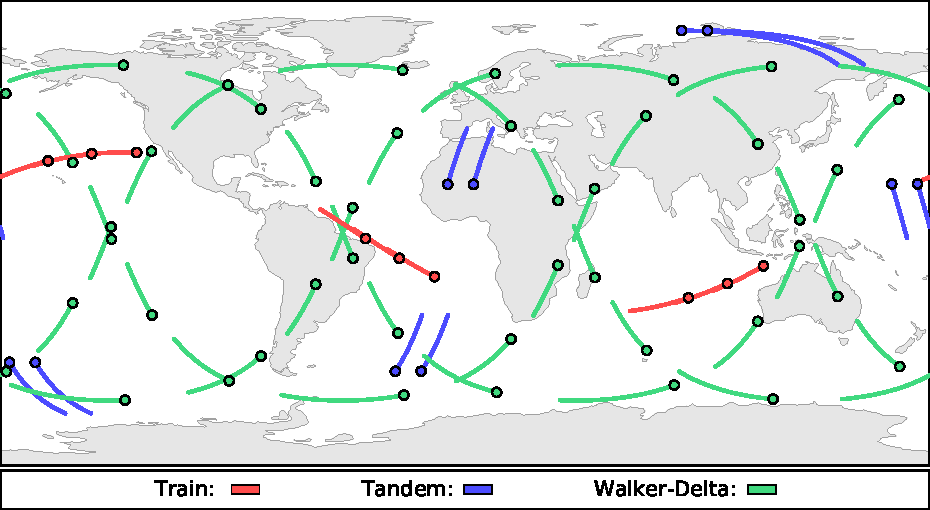
\includegraphics[width=0.6\textwidth]{./images/constellations.pdf}
\end{center}

Sensor hardware is attached to satellites as an interface to truth data (NetCDF
Nature Run data).  This provides a custom modeling environment for real sensor
hardware and enables heterogeneous sensor constellations with different
capabilities.  As a satellite orbits, its pointing vector intersects Earth's
surface or an atmospheric layer and samples the underlying data.

\begin{center}
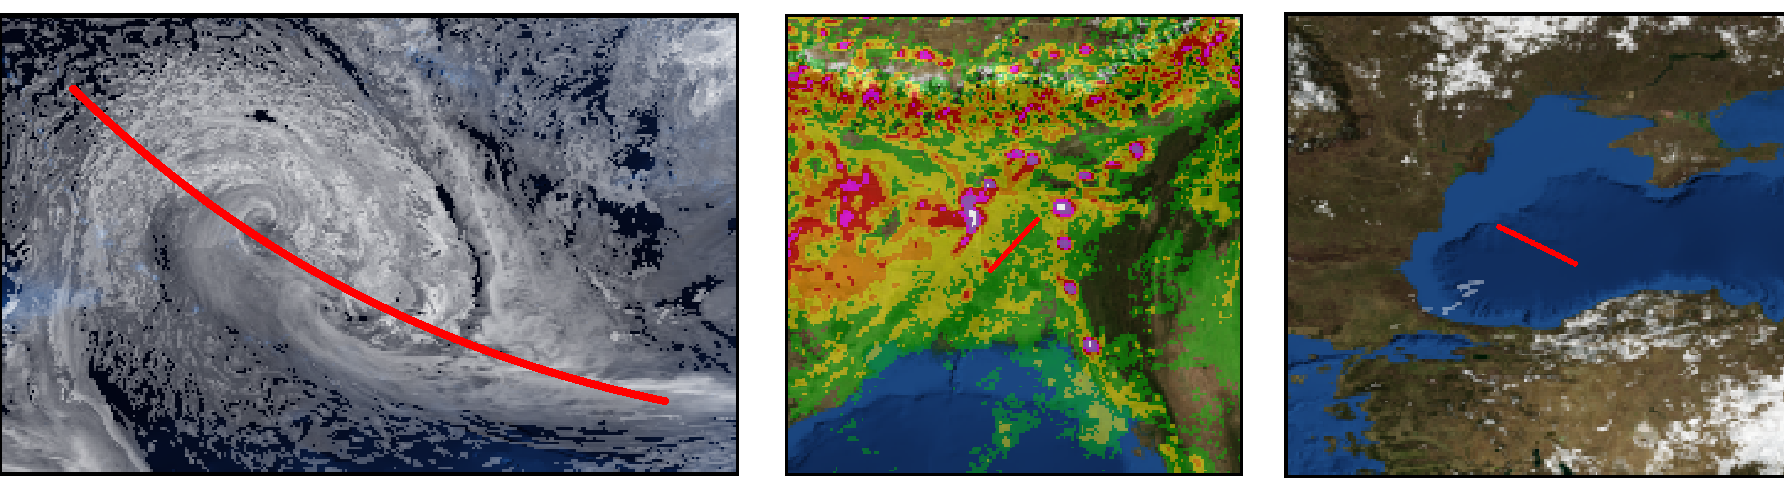
\includegraphics[width=0.6\textwidth]{./images/remote_sensing.pdf}
\end{center}

Collaborate is named for its ability to manage collaborative networks of
satellites.  Its implementation focuses on the high-level communication decision
space previously discussed.  The library employs, in addition to standard C++
components, advanced data structures including trees and graphs to execute
predictive route-finding algorithms for efficient communications.

\begin{center}
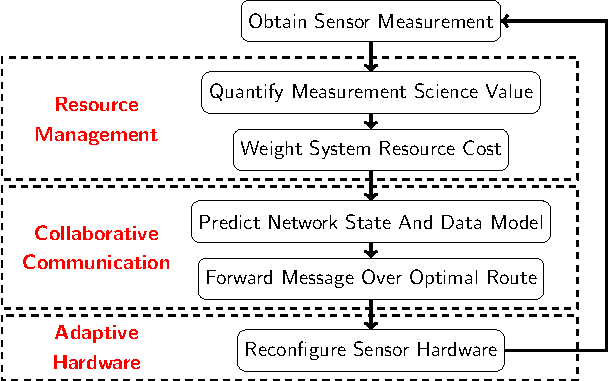
\includegraphics[width=0.5\textwidth]{./images/flowchart.pdf}
\end{center}

\begin{center}
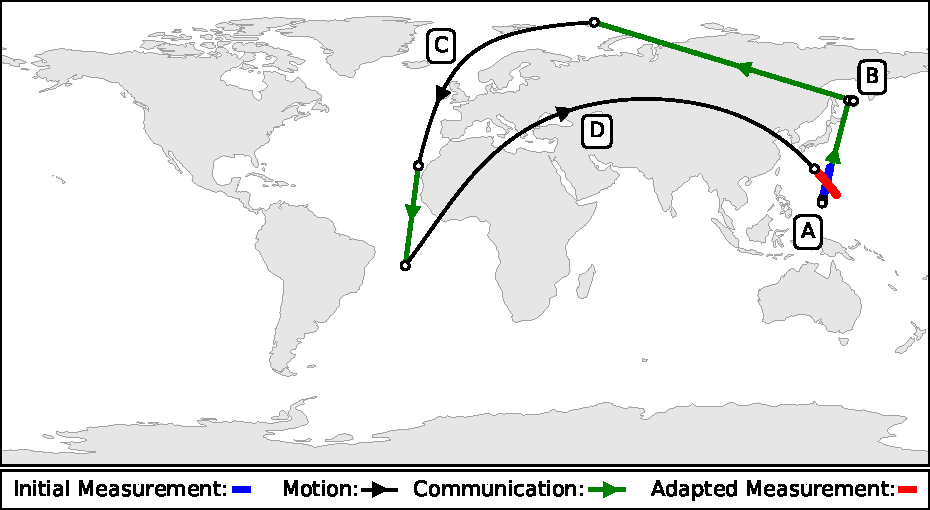
\includegraphics[width=0.6\textwidth]{./images/collaborate.pdf}
\end{center}

These network algorithms are the highlight of project development because they
expedite two valuable capabilities for researching cognitive behavior and
machine learning applications.  First, Collaborate's networking algorithms
provide a feedback mechanism to satellites executing deployed machine learning
algorithms.  Second, Collaborate produces verbose simulation data which can be
used to train neural networks and other machine learning models.

In addition to forward propogation of data, satellites can feed back relevant
information to the original satellite for regression tasks.  This is useful when
optimizing low-level communication parameters, learning the correlation between
truth data parameters, or to promote sensor hardware reconfiguration.

\begin{center}
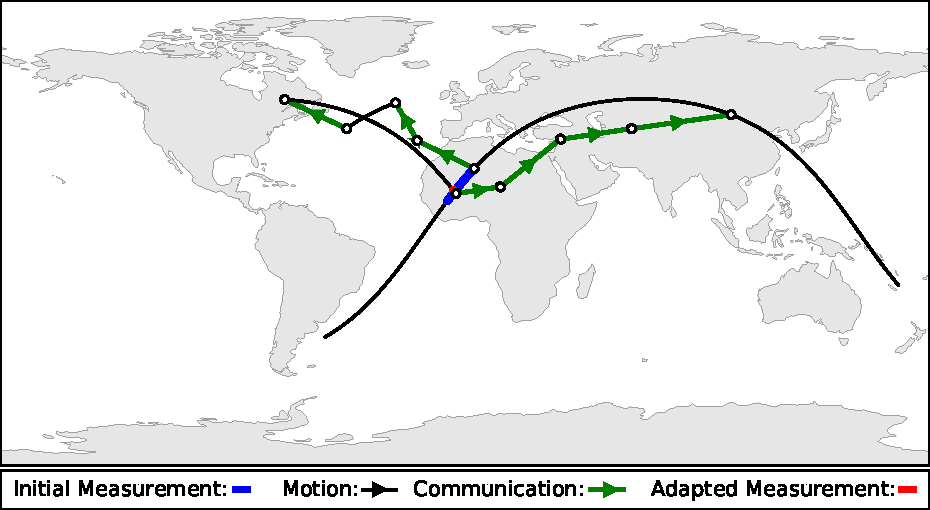
\includegraphics[width=0.6\textwidth]{./images/loop.pdf}
\end{center}

\begin{center}
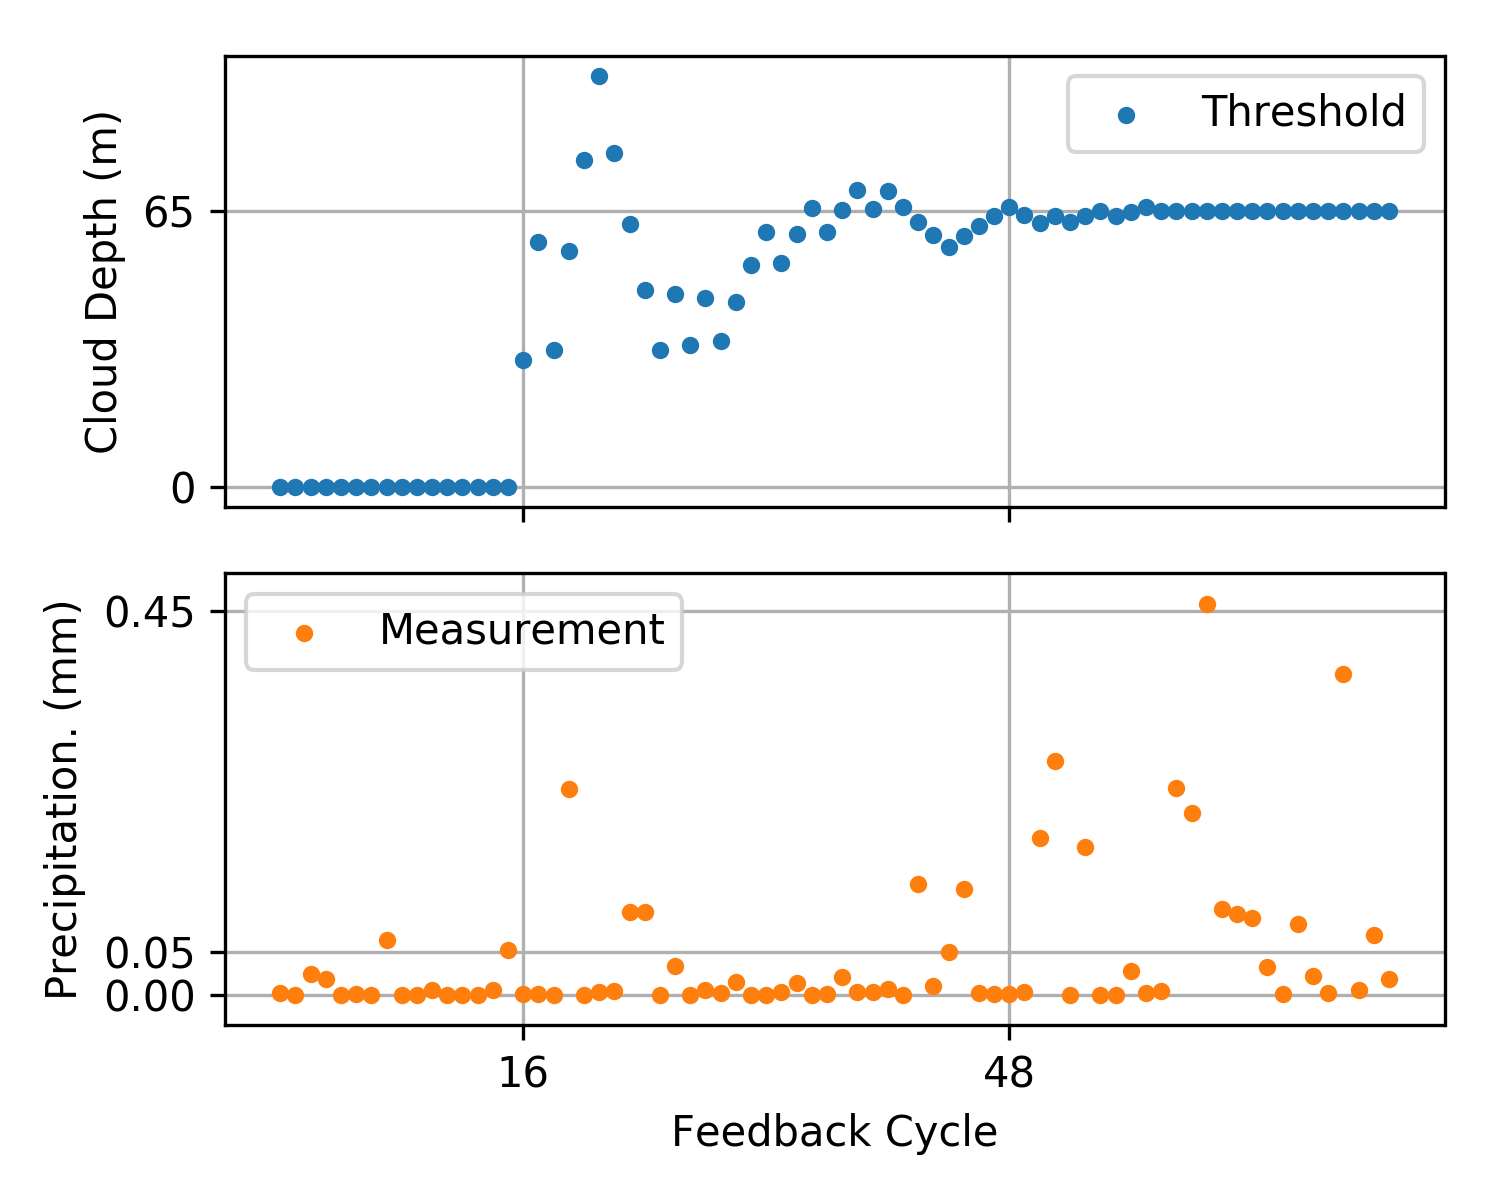
\includegraphics[width=0.6\textwidth]{./images/regression.png}
\end{center}

\begin{itemize}
\item Key is that it can output large sets of collaborative and adatpive simulation
results.

\item Using Collborate to generate traning data
\end{itemize}

Collaborate logs simulation data to files accessible by external machine
learning tools.  The provided Python packages undersand the data format and can
read and store the data for later use as Numpy or Pandas data structures.  Logs
are provided in two main formats: first, a time series of data frames containing
satellite node parameters; second, network connections are stored as adjacency
matrices.

\begin{center}
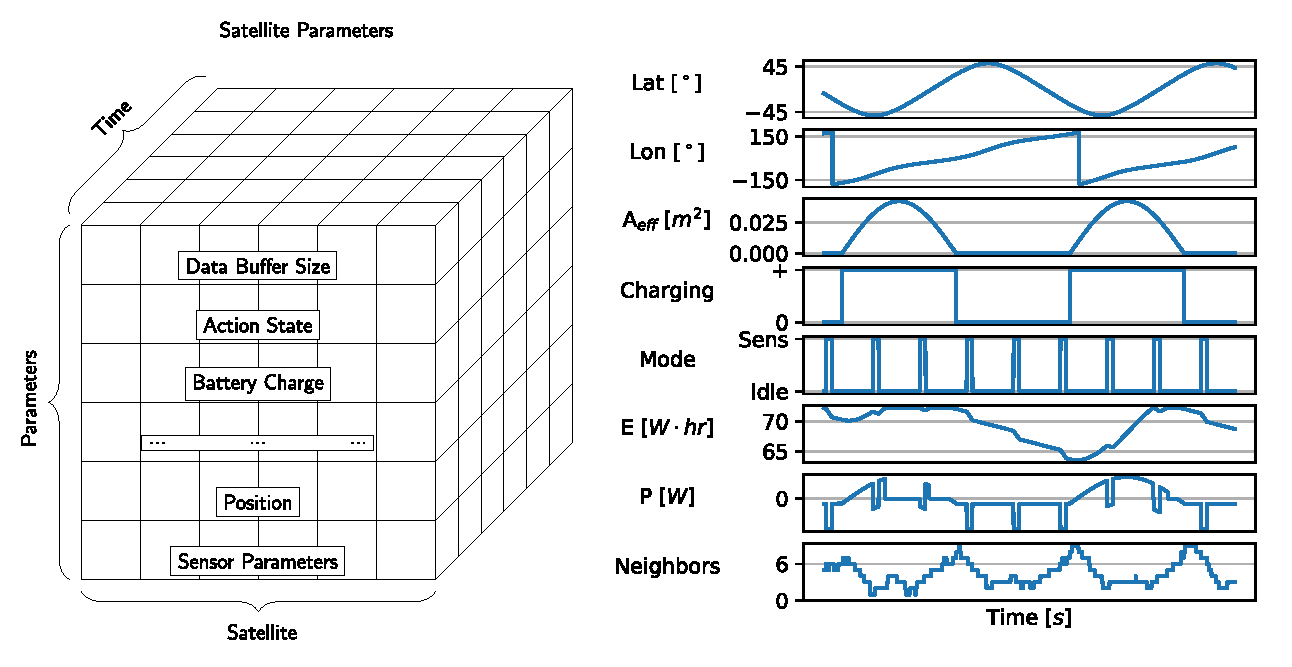
\includegraphics[width=\textwidth]{./images/parameters_combined.pdf}
\end{center}

\begin{center}
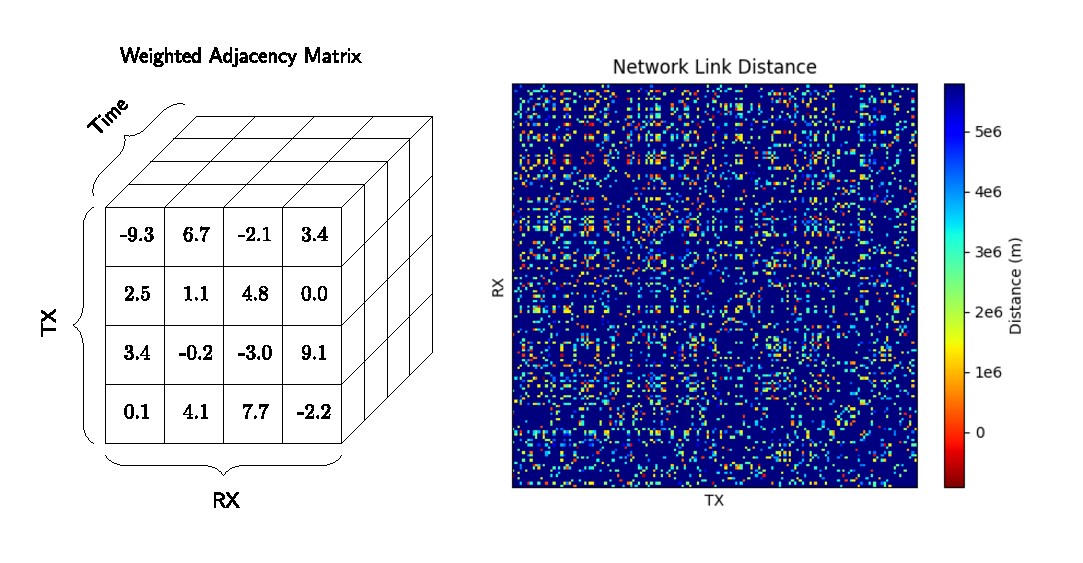
\includegraphics[width=\textwidth]{./images/weighted_combined.pdf}
\end{center}

\begin{itemize}
\item Collaborate simulates complex algorithms that take a long time to execute to
make good decisions

\item Concept will be to replace these algorithms with an efficient NN.

\item What was specifically generated for the case studies \ldots{}
\end{itemize}

\section*{V. EXAMPLE CASE STUDIES}
\label{sec:orgf49f226}

Description of examples and why they were chosen.

\subsection*{A. Example 1}
\label{sec:org09f60a0}

\ldots{}

\subsection*{B. Example 2}
\label{sec:org00fe754}

\ldots{}

\section*{VI. SUMMARY AND NEXT STEPS}
\label{sec:orgb32679a}

\ldots{}

\section*{REFERENCES}
\label{sec:orgc00bb67}

\ldots{}
\end{document}
